%======================================================================
\chapter{Architecture}
%======================================================================
\label{ch:arch}

\begin{figure}[b!]
\centering
  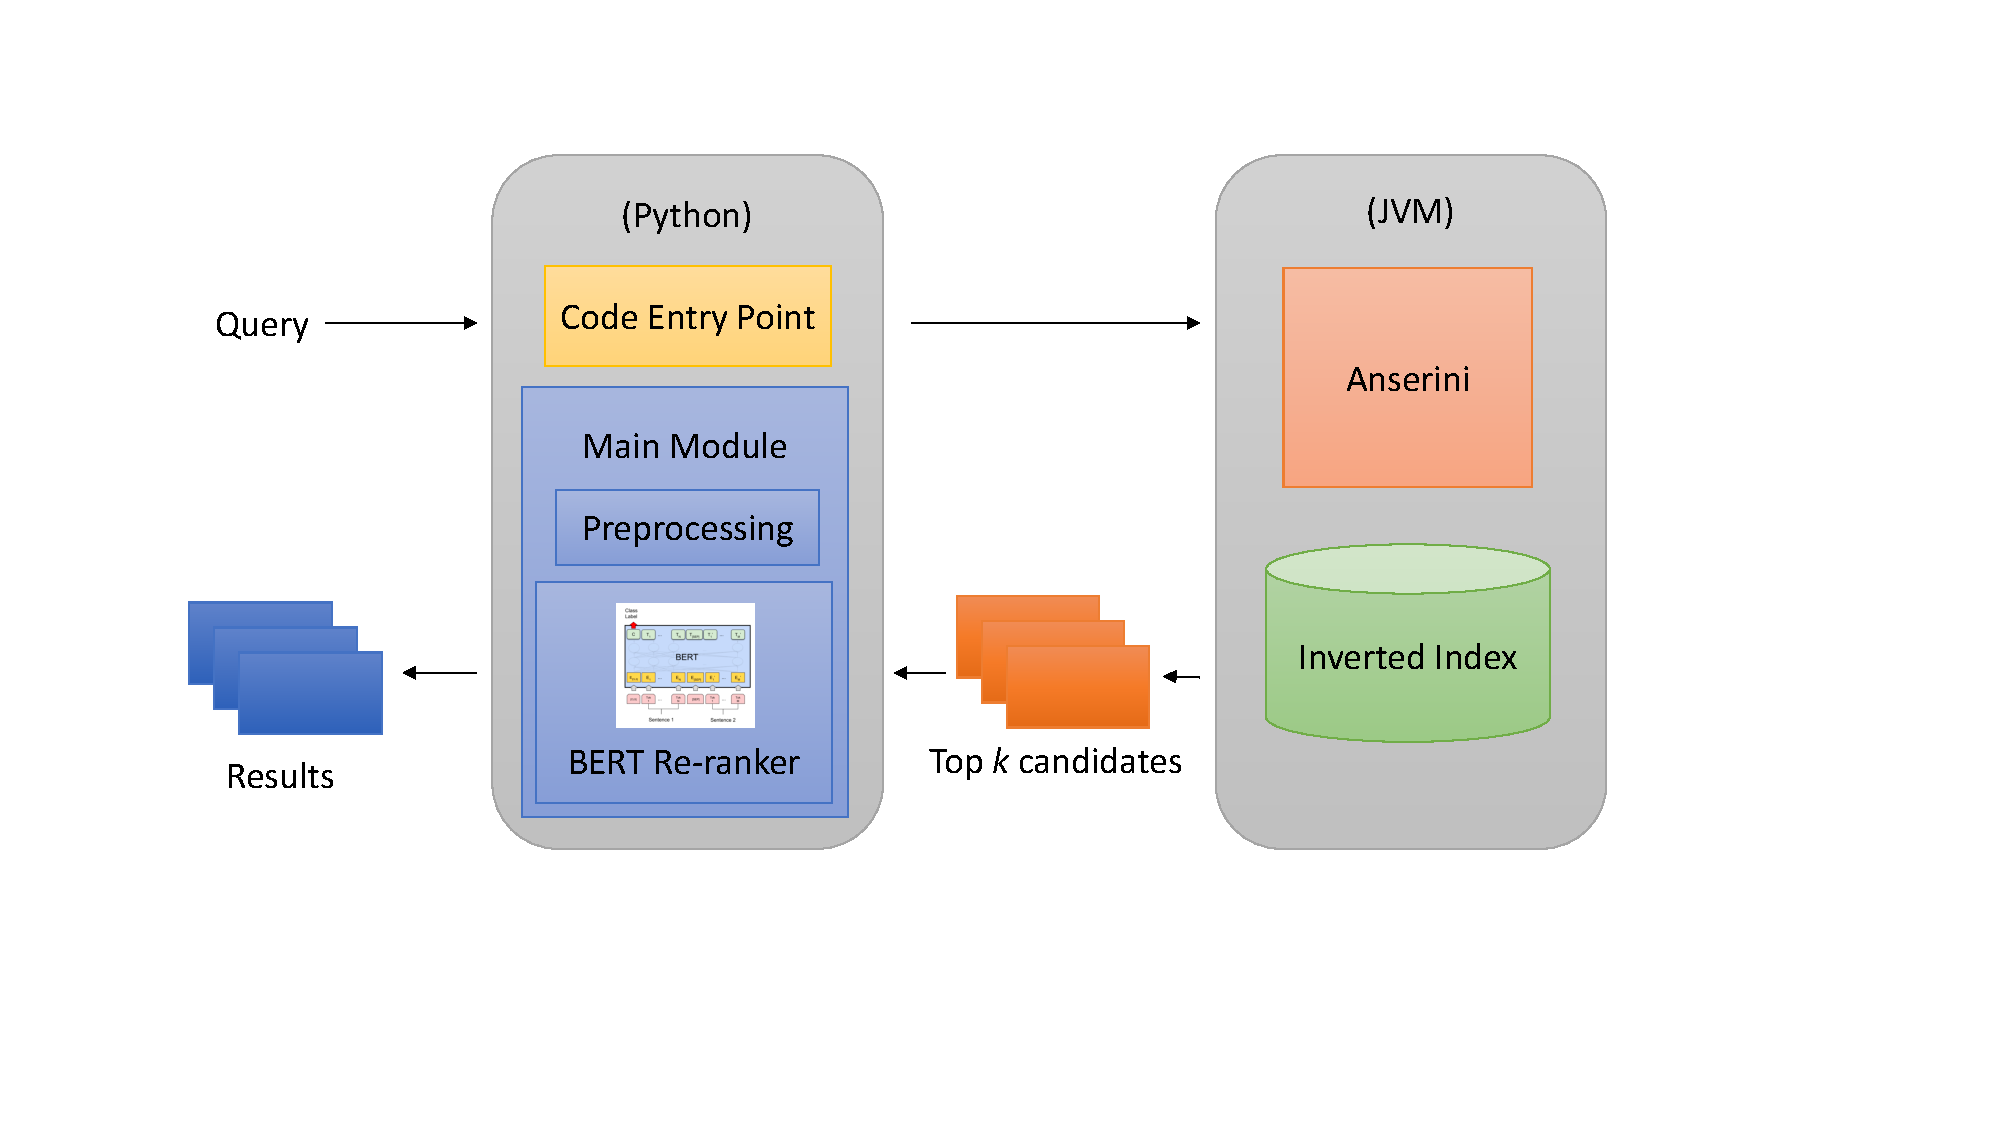
\includegraphics[width=5in]{architecture.pdf}
\caption{...}
\label{fig:arch}
\end{figure}

We apply BERT to document retrieval via integration with an open-source Anserini information retrieval toolkit.
The proposed architecture of our system is composed of a two-stage pipeline where Anserini is responsible for retrieval and a BERT-based reranker consumes the output from Anserini to produce the final ranking of documents.
The individual components of the architecture are shown in Figure \ref{fig:arch}.
These parts can be divided into two main categories based on their medium of execution:\ Python and JVM.

\section{Anserini}

Within the information retrieval community, there exists a gap between academic research and real-world search applications built in the industry.
While a few select organizations, mostly large search companies, deploy custom search infrastructure, most industry practitioners rely on Lucene or the closely related Solr and Elasticsearch as the de facto platform.
On the other hand, academic systems such as Indri\footnote{•} and Terrier\footnote{•} are far more common among researchers.
This disconnect between the two groups hinders technology transfer and potential impact of research results.

To address this gap, Anserini~\cite{} was developed to provide a research-focused information retrieval toolkit on top of the open-source Lucene search library.
Like Lucene, Anserini provides efficient full text indexing and search capabilities over large-scale text collections.
More importantly, Anserini makes it possible for researchers and industry practitioners alike to systematically evaluate their models over standard test collections in a reproducible and comparable manner.
%\myworries{wrappers, extensions?}

Anserini has already been successfully adopted in multiple projects:\
For example, \cite{nogueira2019passage} used Anserini for generating candidate documents before applying BERT to ranking passages in the TREC Complex Answer Retrieval (CAR) task~\cite{dietz2017trec}, which led to a large increase in effectiveness.
\cite{Yang_etal_arXiv2019} also combined Anserini and BERT to demonstrate large improvements in open-domain question answering directly on Wikipedia.

In our architecture, Anserini wrappers are used to index our test collections with Lucene 8.
We then retrieve the initial candidate list of documents from the respective index with Anserini.
\myworries{low-latency, optimized blahblah...}
These documents are then fed into the Python module where they are processed \myworries{what else?}.

\section{Python Module}

Our Python module lies at the crux of the Birch system, encompassing the preprocessing, training and evaluation components.
The preprocessing component takes the  top $ k $ candidate documents as input to convert them into a format that can be used by the main Birch module.
The candidate documents are cleaned as described in Section \myworries{X} and split into sentences with the Stanford Tokenizer.

The main Birch module has two functionalities.
On the one hand, it is used to train BERT as a relevance classifier.
This functionality may also be used independently of the overall pipeline to fine-tune BERT on new collections. 
On the other hand, we can run inference over the output of the preprocessing module with the previously trained models.
The output of this module is a list of sentence relevance scores.
Our deep learning framework of choice for this module is PyTorch in Python.

Last but not least, the evaluation module integrates directly with Anserini.
First, an overall document relevance score is computed for each candidate document from both BM25+RM3 and sentence scores.
The two sets of scores are combined to obtain an overall document score.
\myworries{trec eval and Anserini}

\section{Integration}

Integration of NLP and IR capabilities poses a number of technical challenges due to different underlying infrastructures.
In this section we discuss our design choices to bridge the worlds of NLP and IR.
We employ a multi-stage architecture where we retrieve an initial list of candidate documents with Anserini over a standard inverted index, and then re-rank these documents based on BERT sentence scores. 
Built on top of Lucene, Anserini runs on the Java Virtual Machine (JVM) as it is mostly written in Java, or provides Python wrappers on Java.
However, most deep learning toolkits today, including our choice PyTorch, are written in Python with a C\texttt{++} backend.

Bridging Python and the JVM presents a technical challenge that needs to be address for an effective integration.
There exist two immediate solutions to address this problem.
``Loosely-coupled'' integration approaches involve using an intermediary medium between Python and the JVM.
For example, we may pass intermediate text files between the two in order to facilitate communication without direct interaction.
However, this is not an efficient solution as it requires writing and reading potentially large files to disk, not to mention the memory requirements.
Furthermore, this approach requires constant diligent monitoring to ensure that changing file formats and APIs do not break code.
Integration via REST APIs is plagued with similar issues.
This approach may require frequent HTTP calls that introduce significant overhead.
Additionally, imperfect solutions for enforcing API contracts risk stability of the system.
Neither approach is suitable for rapid experimentation in a research environment.

Therefore, we explore ways to achieve ``tightly-coupled'' integration.
One solution is to adopt the Java Virtual Machine (JVM) as the primary code entry point, and connect to the Torch backend via the Java Native Interface (JNI).
\myworries{How?}
However, this creates two separate code paths (JVM to C\texttt{++} for execution and Python to C\texttt{++} for model development), leading to maintainability issues.
For this reason, we finally chose Python as our primary development environment, integrating Anserini using the Pyjnius Python library\footnote{\url{https://pyjnius.readthedocs.io/}} for accessing Java classes.
Pyjnius was originally developed to facilitate Android development in Python, and allows Python code to directly manipulate Java classes and objects.
Thus, Birch supports Python as the main development language (and code entry point, as shown in Figure~\ref{fig:arch}), connecting to the backend JVM to access retrieval capabilities.

\section{Reproducibility}

Over the last decade, it has become increasingly challenging to verify reported results and compare various performance metrics due to growing number of information retrieval systems both in academia and industry alike.
Unlike some research fields where it is practical to manually corroborate findings or visually inspect results, the amount and type of data involved in document retrieval deems this approach infeasible.
As a matter of fact, this issue has attracted so much attention in the community that one of the biggest IR conferences in the world, SIGIR, has recently issued a task force to determine guidelines to implement repeatability, replicability and reproducibility principles in IR projects.\footnote{http://sigir.org/wp-content/uploads/2018/07/p004.pdf}

The first dimension of this movement, repeatability, emphasises a researcher's ability to reliably repeat her own computation.
The path to this goal is through rigorous logging, good data management practices and consistent use of virtual environments.
A number of frameworks that help machine learning researchers keep track of their experiments, such as Sacred\footnote{https://github.com/IDSIA/sacred} and Forge\footnote{https://github.com/akosiorek/forge}, have emerged over the last few years.
By adding only a few lines of code, these frameworks save and display the details of each experiments on an online dashboard so that the researcher can go back and reproduce her experiments easily.

The second dimension, replicability, instead highlights the ability of an independent group to obtain the same results using the author's original artifacts.
To this end, we build a Docker image to accompany our system that allows anyone to deploy and test our system on any operating system easily.
By adhering to the requirements defined in the SIGIR Open-Source IR Replicability Challenge (OSIRRC), we ensure that our system can seamlessly work with their evaluation infrastructure in the future.
The image is available on Docker hub with the tag \myworries{tag}.
The OSIRRC jig\footnote{https://github.com/osirrc/jig} needs to be set up first to run the commands on Docker hub.
The OSIRRC Docker container contract includes three ``hooks'' for interacting with the system:\
The \texttt{init} hook has to be called first, whose purpose is to run any preparatory steps for the retrieval run including downloading and compiling the source code, downloading pre-built artifacts such as JAR files and other external resources such as pretrained models.
In our case, we pull the source code, data and pretrained models from Google Cloud Storage buckets; build Anserini with Maven, and the TREC evaluation tool.
Next the \texttt{index} hook is called to, as the name indicates, build the necessary indexes.
Finally, the \texttt{search} hook helps perform multiple ad-hoc retrieval runs in a row.
Each of the hook scripts accepts a JSON file that defines the various arguments for the respective script such as path to the relevance judgements file.
Similar to the Google Colab notebook, the Docker image is restricted to experiments with $ \textrm{BERT}_{\textrm{\scriptsize Base}}(\textrm{MB})$ on Robust04 for the sake of simplicity.

Finally, the third dimension, reproducibility refers to the case where an independent group of researchers implements the author's proposed artifacts from scratch with the same results.
This final goal is indeed the hardest to achieve; as a matter of fact, it may even be impossible in certain cases due to non-determinism.
For example, the fine-tuning process described in Section \ref{model} produces slightly different sentence scores every time it is performed.
Fortunately for this architecture, these differences in score become negligible after re-ranking.
However, in the general case, the researcher must strive to describe the experimental setup thoroughly in her publications, and open-source her source code whenever possible for reproducibility.

\myworries{Talk about Birch non-determinism and other crap, hyperparameters}
\myworries{Demo stuff?}